%%%%%%%%%%%%%%%%%%%%%%%%%%%%%%%%%%%%%%%%%
% Masters/Doctoral Thesis
% LaTeX Template
% Version 2.5 (27/8/17)
%
% This template was downloaded from:
% http://www.LaTeXTemplates.com
%
% Version 2.x major modifications by:
% Vel (vel@latextemplates.com)
%
% This template is based on a template by:
% Steve Gunn (http://users.ecs.soton.ac.uk/srg/softwaretools/document/templates/)
% Sunil Patel (http://www.sunilpatel.co.uk/thesis-template/)
%
% Template license:
% CC BY-NC-SA 3.0 (http://creativecommons.org/licenses/by-nc-sa/3.0/)
%
%%%%%%%%%%%%%%%%%%%%%%%%%%%%%%%%%%%%%%%%%

%----------------------------------------------------------------------------------------
%	PACKAGES AND OTHER DOCUMENT CONFIGURATIONS
%----------------------------------------------------------------------------------------

% Pages (from the internal page numbering) to be printed in color - 3, 4, 5, 11, 12, 13, 14, 17, 18, 20, 21, 23, 25, 27.

\documentclass[
hidelinks,
12pt, % The default document font size, options: 10pt, 11pt, 12pt
oneside, % Two side (alternating margins) for binding by default, uncomment to switch to one side
english, % ngerman for German
doublespacing, % Single line spacing, alternatives: onehalfspacing or singlespacing
%draft, % Uncomment to enable draft mode (no pictures, no links, overfull hboxes indicated)
%nolistspacing, % If the document is onehalfspacing or doublespacing, uncomment this to set spacing in lists to single
%liststotoc, % Uncomment to add the list of figures/tables/etc to the table of contents
%toctotoc, % Uncomment to add the main table of contents to the table of contents
%parskip, % Uncomment to add space between paragraphs
%nohyperref, % Uncomment to not load the hyperref package
headsepline, % Uncomment to get a line under the header
%chapterinoneline, % Uncomment to place the chapter title next to the number on one line
%consistentlayout, % Uncomment to change the layout of the declaration, abstract and acknowledgements pages to match the default layout
]{MastersDoctoralThesis} % The class file specifying the document structure

\usepackage[utf8]{inputenc} % Required for inputting international characters
\usepackage[T1]{fontenc} % Output font encoding for international characters
\usepackage{subcaption}
\usepackage{mathpazo} % Use the Palatino font by default
\usepackage{booktabs}
\usepackage{colortbl}
\usepackage[final]{pdfpages}
\usepackage{xcolor}
\usepackage{balance}
\usepackage{epigraph}
\usepackage{alltt} % for code snippet
\usepackage{listings}
\usepackage{hyperref}
\usepackage{amsmath}
%\usepackage{fixltx2e}
\usepackage[backend=bibtex,style=authoryear,natbib=true]{biblatex} % Use the bibtex backend with the authoryear citation style (which resembles APA)
\usepackage{float}
\restylefloat{table}

\addbibresource{biblio.bib} % The filename of the bibliography


%\usepackage[autostyle=true]{csquot\right) es} % Required to generate language-dependent quotes in the bibliography

\newcommand{\Pa}{PaO\textsubscript{2}~}
\newcommand{\Sp}{SpO\textsubscript{2}~}
\newcommand{\Fi}{FiO\textsubscript{2}~}
\newcommand{\PF}{PaO\textsubscript{2}/\Fi ratio~}
\newcommand{\SF}{SpO\textsubscript{2}/\Fi ratio~}

%----------------------------------------------------------------------------------------
%	MARGIN SETTINGS
%----------------------------------------------------------------------------------------

\geometry{
	paper=a4paper, % Change to letterpaper for US letter
	inner=4.0cm, % Inner margin
	outer=3.0cm, % Outer margin
	bindingoffset=.5cm, % Binding offset
	top=2.5cm, % Top margin
	bottom=2.5cm, % Bottom margin
	%showframe, % Uncomment to show how the type block is set on the page
}

%----------------------------------------------------------------------------------------
%	THESIS INFORMATION
%----------------------------------------------------------------------------------------

\thesistitle{SpO\textsubscript{2}/FiO\textsubscript{2} ratio (SF ratio) as a predictor of mortality in ICU patients: Retrospective
study using MIMIC Database.} % Your thesis title, this is used in the title and abstract, print it elsewhere with \ttitle
\supervisor{Dr.Willem \textsc{van den Boom}} % Your supervisor's name, this is used in the title page, print it elsewhere with \supname
\examiner{Dr/Pr. FirstName \textsc{LastName}} % Your examiner's name, this is not currently used anywhere in the template, print it elsewhere with \examname
\degree{B.Sc (Hons)} % Your degree name, this is used in the title page and abstract, print it elsewhere with \degreename
\author{Ahmed \textsc{Gobba}} % Your name, this is used in the title page and abstract, print it elsewhere with \authorname
\addresses{} % Your address, this is not currently used anywhere in the template, print it elsewhere with \addressname

\subject{Mathematical, Computational and Statistical Sciences} % Your subject area, this is not currently used anywhere in the template, print it elsewhere with \subjectname
\keywords{Insert, keywords, here} % Keywords for your thesis, this is not currently used anywhere in the template, print it elsewhere with \keywordnames
\university{\href{https://www.yale-nus.edu.sg/}{Yale-NUS College}} % Your university's name and URL, this is used in the title page and abstract, print it elsewhere with \univname
\department{{}} % Your department's name and URL, this is used in the title page and abstract, print it elsewhere with \deptname
\group{{}} % Your research group's name and URL, this is used in the title page, print it elsewhere with \groupname
\faculty{{}} % Your faculty's name and URL, this is used in the title page and abstract, print it elsewhere with \facname

\AtBeginDocument{
\hypersetup{colorlinks=false}
\hypersetup{pdftitle=\ttitle} % Set the PDF's title to your title
\hypersetup{pdfauthor=\authorname} % Set the PDF's author to your name
\hypersetup{pdfkeywords=\keywordnames} % Set the PDF's keywords to your keywords
}

\begin{document}
\sloppy 
\frontmatter % Use roman page numbering style (i, ii, iii, iv...) for the pre-content pages

\pagestyle{plain} % Default to the plain heading style until the thesis style is called for the body content

%----------------------------------------------------------------------------------------
%	TITLE PAGE
%----------------------------------------------------------------------------------------

\begin{titlepage}
% Fill out the titlepage.docx document, then save it as a pdf for inclusion here
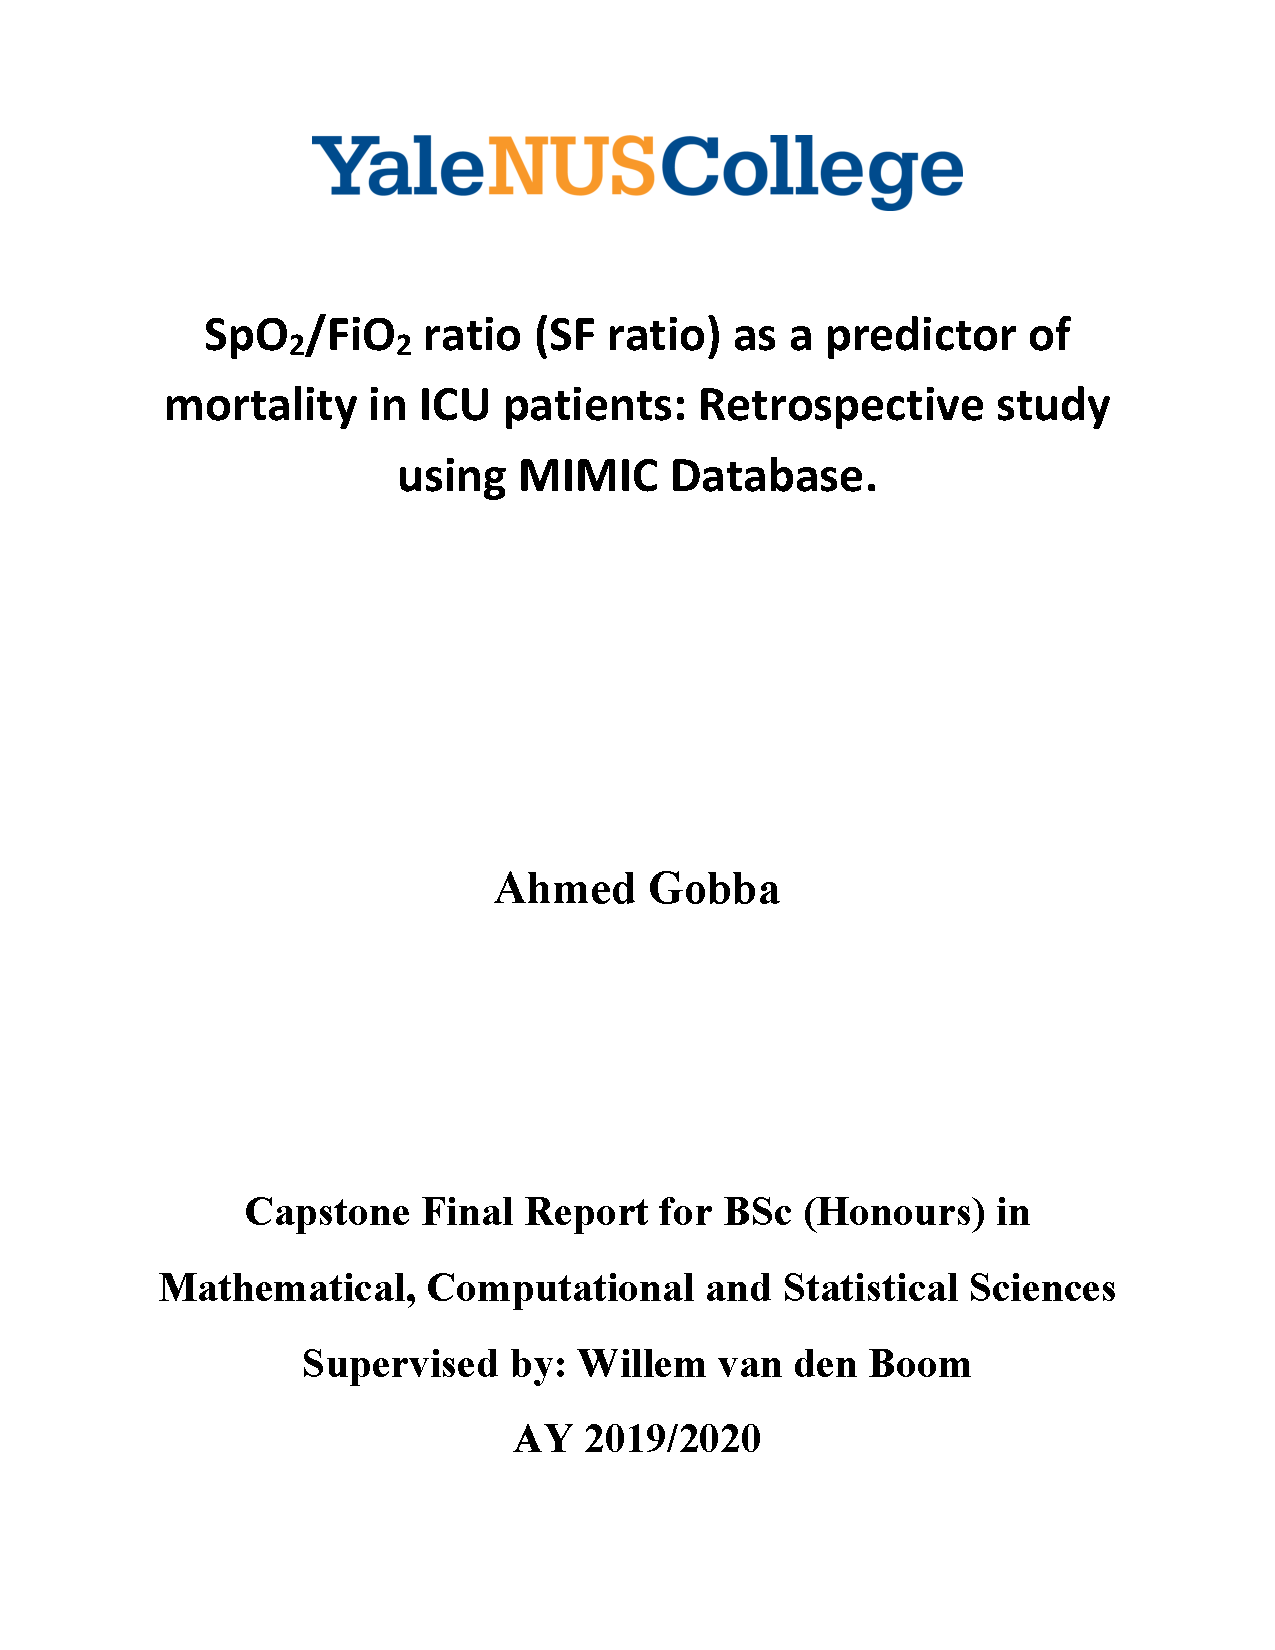
\includepdf[pages=-,pagecommand={},width=\textwidth]{titlepage.pdf}

\end{titlepage}

%----------------------------------------------------------------------------------------
%	DECLARATION & CONSENT
%----------------------------------------------------------------------------------------

% print, sign, and scan the declaration form, then include it here
%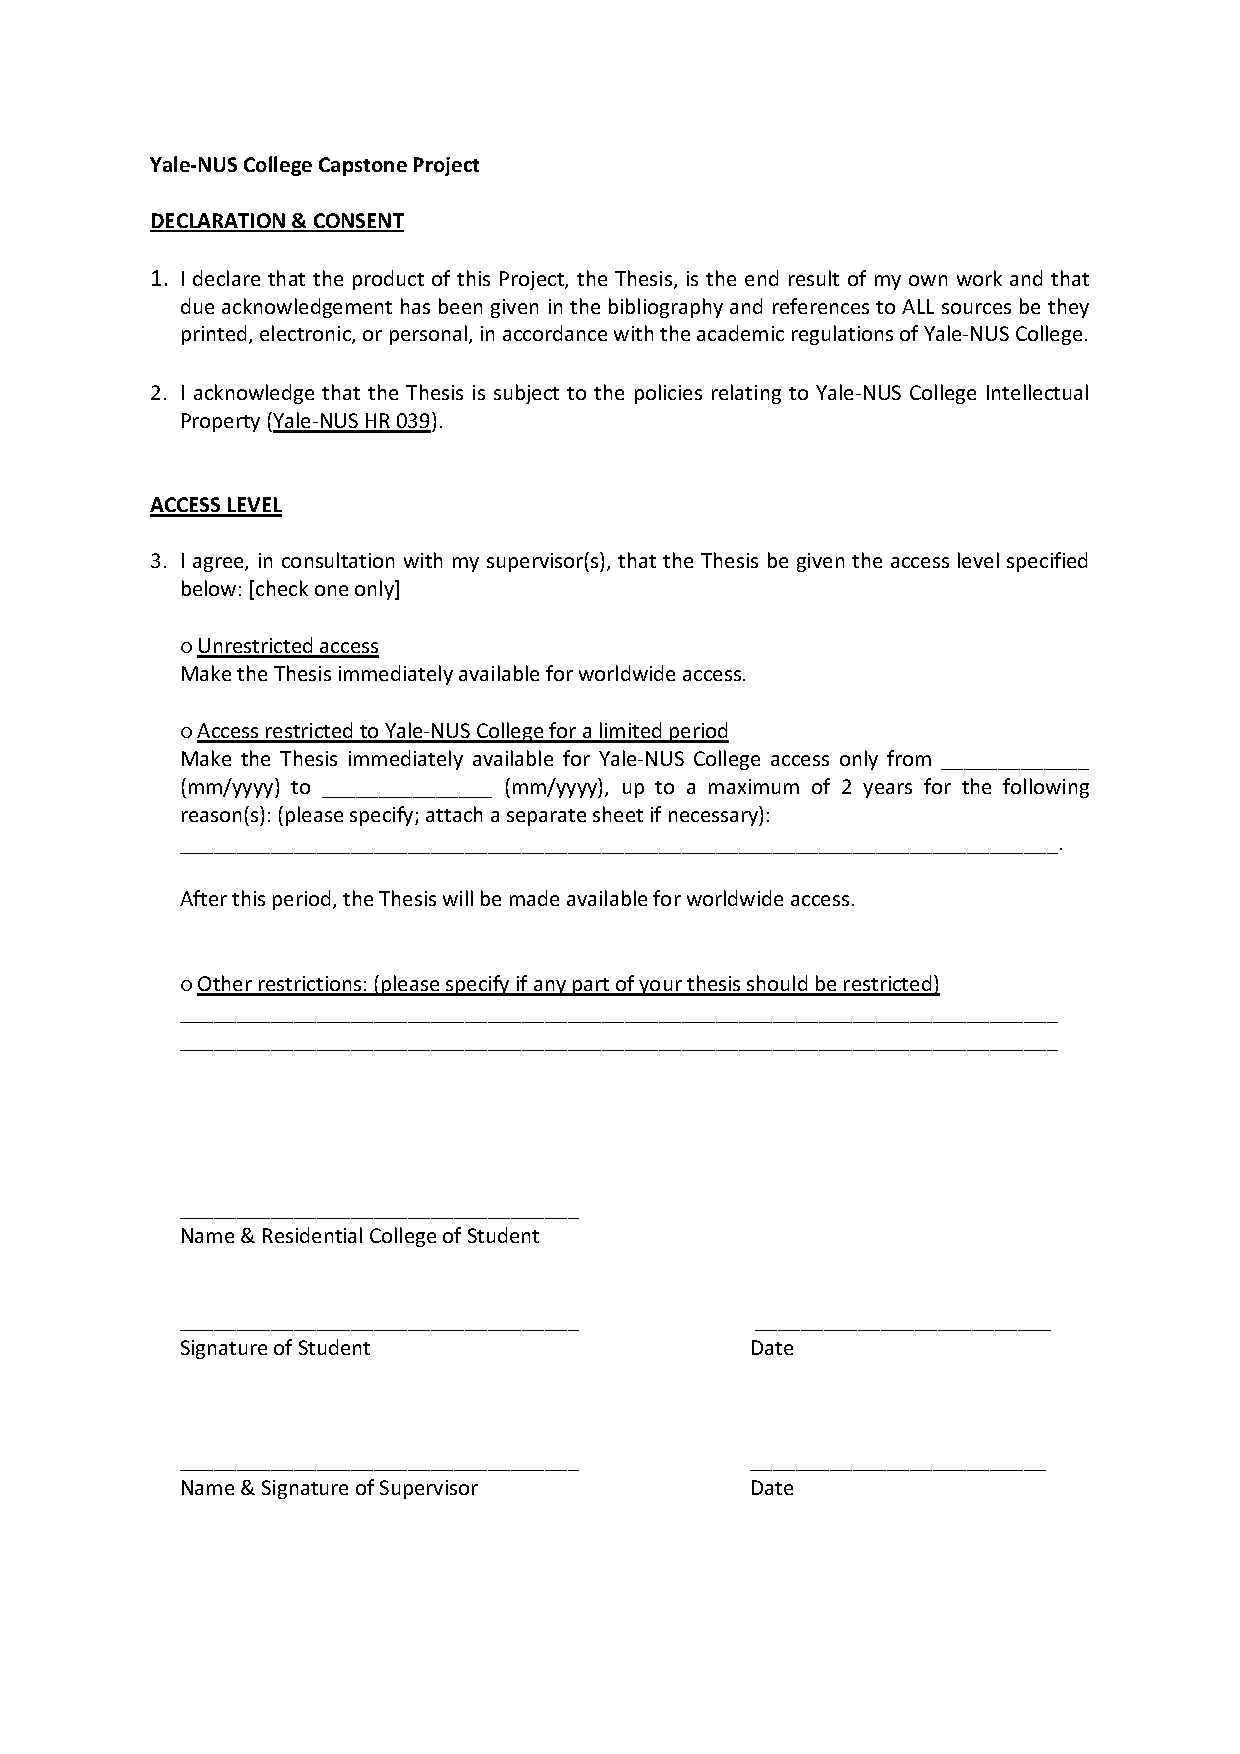
\includepdf[pages=-,pagecommand={},width=\textwidth]{declaration.pdf}

%----------------------------------------------------------------------------------------
%	ACKNOWLEDGEMENTS
%----------------------------------------------------------------------------------------

%\begin{acknowledgements}
%\addchaptertocentry{\acknowledgementname} % Add the acknowledgements to the table of contents
%Acknowledgements go here.
%\end{acknowledgements}

%----------------------------------------------------------------------------------------
%	ABSTRACT PAGE
%----------------------------------------------------------------------------------------

%\begin{abstract}
%\addchaptertocentry{\abstractname} % Add the abstract to the table of contents
%Abstract goes here.
%\end{abstract}


%----------------------------------------------------------------------------------------
% CONTRIBUTIONS
%----------------------------------------------------------------------------------------

% \chapter{Claims}
%
% This paper presents the following original contributions:
%
% \begin{enumerate}
% 	\item A hardware device for haptic sensory substitution along with designs for the construction of such a system.
% 	\item Two implementations of sensory substitution using haptic feedback, continuous and delayed feedback-based spatial navigation tasks, each of which include:
% 		\begin{enumerate}
% 			\item a front-end for providing visual input to the user during the training phase with useful readouts to the researcher,
% 			\item a transmission protocol, which maps information from the task at hand (spatial coordinates, velocity information, etc) to time-based sensor actuation signals (20$^{\circ}$ on servo 1, 35$^{\circ}$ on servo 2, etc) in real-time.
% 		\end{enumerate}
% 	\item An evaluation framework for measuring the performance of a sensory substitution system, which provides sample tasks that can be used to standardise and compare performance across the board for future research.
% 	\item A review of existing hardware and software stacks as well as possible avenues for development based on the developed metrics.
% \end{enumerate}
%
% In addition, code for displaying results in real-time, modules for managing servo overload, network latency and other factors were also written by the author.


% %----------------------------------------------------------------------------------------
% %	DECLARATION PAGE
% %----------------------------------------------------------------------------------------
%
% \begin{declaration}
% \addchaptertocentry{\authorshipname} % Add the declaration to the table of contents
%
% \noindent I, \authorname, hereby declare that this Project, the Capstone Report and associated work listed herein, is the end result of my own work and that due acknowledgement has been given in the bibliography and references to ALL sources printed, electronic, or personal, in accordance with the academic regulations of Yale‐NUS College.
% I acknowledge that the Thesis is subject to the policies relating to Yale‐NUS College Intellectual  Property (Yale‐NUS HR 039).
%
%
% % I confirm that:
% %
% % \begin{itemize}
% % \item This work was done wholly or mainly while in candidature for a research degree at this University.
% % \item Where any part of this thesis has previously been submitted for a degree or any other qualification at this University or any other institution, this has been clearly stated.
% % \item Where I have consulted the published work of others, this is always clearly attributed.
% % \item Where I have quoted from the work of others, the source is always given. With the exception of such quotations, this thesis is entirely my own work.
% % \item I have acknowledged all main sources of help.
% % \item Where the thesis is based on work done by myself jointly with others, I have made clear exactly what was done by others and what I have contributed myself.\\
% % \end{itemize}
%
% \noindent Signed:\\
% \rule[0.5em]{25em}{0.5pt} % This prints a line for the signature
%
% \noindent Date:\\
% \rule[0.5em]{25em}{0.5pt} % This prints a line to write the date
% \end{declaration}
%
% \cleardoublepage

%----------------------------------------------------------------------------------------
%	QUOTATION PAGE
%----------------------------------------------------------------------------------------

% \vspace*{0.2\textheight}
%
% \noindent\enquote{\itshape Thanks to my solid academic training, today I can write hundreds of words on virtually any topic without possessing a shred of information, which is how I got a good job in journalism.}\bigbreak
%
% \hfill Dave Barry

%----------------------------------------------------------------------------------------
%	LIST OF CONTENTS/FIGURES/TABLES PAGES
%----------------------------------------------------------------------------------------

\tableofcontents % Prints the main table of contents

%\listoftables % Prints the list of tables
%\label{lst:tabs}

%\listoffigures % Prints the list of figures
%\label{lst:figs}
%----------------------------------------------------------------------------------------
%	ABBREVIATIONS
%----------------------------------------------------------------------------------------

% \begin{abbreviations}{ll} % Include a list of abbreviations (a table of two columns)
%
% \textbf{LAH} & \textbf{L}ist \textbf{A}bbreviations \textbf{H}ere\\
% \textbf{WSF} & \textbf{W}hat (it) \textbf{S}tands \textbf{F}or\\
%
% \end{abbreviations}

%----------------------------------------------------------------------------------------
%	PHYSICAL CONSTANTS/OTHER DEFINITIONS
%----------------------------------------------------------------------------------------

% \begin{constants}{lr@{${}={}$}l} % The list of physical constants is a three column table
%
% % The \SI{}{} command is provided by the siunitx package, see its documentation for instructions on how to use it
%
% Speed of Light & $c_{0}$ & \SI{2.99792458e8}{\meter\per\second} (exact)\\
% %Constant Name & $Symbol$ & $Constant Value$ with units\\
%
% \end{constants}

%----------------------------------------------------------------------------------------
%	SYMBOLS
%----------------------------------------------------------------------------------------

% \begin{symbols}{lll} % Include a list of Symbols (a three column table)
%
% $a$ & distance & \si{\meter} \\
% $P$ & power & \si{\watt} (\si{\joule\per\second}) \\
% %Symbol & Name & Unit \\
%
% \addlinespace % Gap to separate the Roman symbols from the Greek
%
% $\omega$ & angular frequency & \si{\radian} \\
%
% \end{symbols}

%----------------------------------------------------------------------------------------
%	DEDICATION
%----------------------------------------------------------------------------------------

%\dedicatory{Dedicated to ceux l\`{a} qui veulent.}

%----------------------------------------------------------------------------------------
%	THESIS CONTENT - CHAPTERS
%----------------------------------------------------------------------------------------

\mainmatter % Begin numeric (1,2,3...) page numbering

\pagestyle{thesis} % Return the page headers back to the "thesis" style

% Include the chapters of the thesis as separate files from the Chapters folder
% Uncomment the lines as you write the chapters

% Chapter 1

\chapter{Clinical Background} % Main chapter title

\label{chapter1} % For referencing the chapter elsewhere, use \ref{Chapter1}


\section{Importance of Biomarkers in ICU Studies}

Allocation of resources to patients to minimize mortality is a constant priority for healthcare professionals. This is especially important in the area of healthcare we have chosen to focus on in this paper: critical care,  where resources such as equipment and attention of specialists are even more scarce. A critical care specialist focuses on the most vulnerable and urgent patients who are placed in an Intensive Care Unit (ICU). In this setting, the specialist is often faced with difficult decisions of which patients to allocate resources to. An unfortunate reminder that has recently put such decisions under the spotlight is the current COVID-19 global pandemic. A recent study on ICU capacity in Wuhan, the disease's epicentre in China, states that at a point during the current crisis the number of COVID-19 patients who need ICU resources is 1120 while only 600 ICU beds existed. As a result, only 25\% of the patients who had died by the time of the study received the intubation and mechanical ventilation that they required \citep{wu2020characteristics}. In Lombardy, the disease's epicentre in Italy, a study states that under pre-crisis conditions,  the city's  total ICU capacity of 720 already operates at 85\% - 90\% during winter months. To make things worse, during the first two weeks after the city's first confirmed COVID-19 case, the number of COVID-19 related ICU admissions rose exponentially to 556. Moreover, estimates for the total number of COVID-19 ICU admissions in the following two weeks suggest an even more drastic shortage with linear estimates at 869 and exponential estimates at 14,542 \citep{grasselli2020}. Hence, ICU capacities are stressed under normal conditions and even further during times of crises.  Faced with such a perpetual dilemma of resource allocation, a critical care specialist uses various biomarkers in order to try and predict severe outcomes in the patients cohort. As such, a persistent priority in medical research is the discovery and analysis of connections between various biomarkers and unfavourable patient outcomes. 

\section{Problem: PF Ratio is an Important but Challenging Biomarker}

One such biomarker that is tracked in ICU settings is the  \PF(PF ratio). It is used to monitor the patient's pulmonary functions. The numerator, \Pa refers to the partial pressure of oxygen in arterial blood. It is measured in mmHg via drawing a sample of blood from an artery in the wrist or groin, and testing it in the laboratory. The denominator, \Fi refers to the initial fraction of inspired oxygen and is approximately 21\% in breathable atmospheric air. In an ICU, it can be controlled by providing the patient with a form of oxygen therapy through to the use of devices such as mechanical ventilators. The PF ratio is most notably used in the diagnosis of extreme illnesses such as Acute Respiratory Distress Syndrome (ARDS) \citep{bernard1994american}. Moreover, it has been shown to be a significant identifier of mortality risk the general ICU population \citep{villar2011risk} and as a predictor of mortality in specific subsets of patients such as newborns with Meconium Aspiration Syndrome (MAS)  \citep{narayanan2019pao2} and post-operation cardiac surgery patients \citep{esteve2014evaluation}.

However, there is a major challenge associated with the use of \Pa - its measurement. The  procedure is invasive and delayed, making it not feasible to track \Pa at frequent intervals measure for all patients. 


\section{Motivation: Can SF Ratio be an Alternative to PF Ratio and for who?}
A more convenient biomarker to measure, however, is \Sp  or peripheral capillary oxygen saturation. It is defined as the ratio of oxygenated haemoglobin by the total amount of haemoglobin in the blood. It is measured using pulse oximetry which uses the principle that oxygenated and deoxygenated haemoglobin have different absorption spectra at particular wavelengths of light \citep{jubran1999pulse} . The oximeter illuminates light at specific wavelengths through the skin (usually at the fingertips) and almost instantaneously calculates the ratio of absorption of these wavelengths to extrapolate the proportion of oxygenated haemoglobin in the blood, or \Sp \citep{jubran2015}. Therefore, unlike \Pa, \Sp can be measured in a non-invasive and instantaneous manner. 

However, a critical difference between, \Pa and \Sp is that the former a generally more accurate measure of a patient's oxygenation level since it is measured directly from a main artery while the latter is measured at the end of capillaries. Nonetheless, recent studies have shown that \SF (SF ratio) has been shown to be a non-invasive surrogate for \PF to diagnose certain subsets of patients such as children with ALI or ARDS \citep{rice2007comparison} and children with smoke inhalation injury \citep{cambiaso2017correlation}. Moreover, a retrospective study found that the SpO\textsubscript{2}/\Fi Time-at-Risk (SF-TAR), defined as the total time spent with severe hypoxemia (SF ratio $\leq 145$), is not only significantly correlated with hospital mortality for mechanically ventilated patients, but is as good or a better predictor of it than arterial gas-derived measurements of the PF ratio. 

There have also been several studies that aim to link \Sp separately to mortality. In 2015, the Tromsø study concluded that an \Sp $\leq95\%$ is associated with all-cause mortality and mortality caused by pulmonary diseases (over a 10-year follow-up period) after adjusting for sex, age, history of smoking, self-reported diseases and respiratory symptoms, BMI, and CRP concentration. When Forced Expiratory Volume (FEV1) was included as a covariate, the correlation remained significant for mortality due to pulmonary diseases but no longer significant for all-cause mortality \citep{vold2015low}. 

However, not all studies investigating a link between \Sp or \\ \SF and mortality have yielded significant results. A prospectively planned meta-analysis study using participant data from 5 randomized clinical trials (conducted from 2005-2014) of infants born before 28 weeks' gestation period found no significant difference between a lower \Sp target range (85\%-89\%) and a higher \Sp target range (91\%-95\%) on mortality or major disability at a corrected age of 18 to 24 months \citep{askie2018association}. Therefore, it seems that the use of \Sp as a predictor of mortality might not be applicable to all patient phenotypes, with potential for further sub-phenotyping. Such differences between the subpopulation might also be expected for the SF ratio which includes \Sp in the numerator. 


\section{Research Question} 

The main goal of this capstone can be summarized as follows: \\
\textit{ Investigate whether \SF is a statistically significant predictor of mortality in general ICU patient population or subsets thereof using a retrospective analysis of ICU patient records.
}

By focusing on \SF instead of only \Sp, we also implicitly hypothesize that the former is a more helpful predictor as it allows us to account for the different levels of mechanical ventilation that an ICU patient receives. In essence, it allows us to account for the patient's ability to convert inspired oxygen to peripheral oxygen saturation at the tissue level. 


\section{Data}

For this capstone I will be using \textbf{MIMIC III}, an openly available relational database developed by the MIT Lab for Computational Physiology. It contains de-identified data of 61,532 intensive care unit stays: 53,432 stays for adult patients and 8,100 for neonatal patients at the Beth Israel Deaconess Medical Center over the June 2001 - October 2012. It includes demographics, vital signs, laboratory tests, medications, mortality, etc. The database is divided into different tables of data that contain information about a patient's stay and are linked to each via identifiers such as a unique hospital admission ID and a unique patient ID. 



This is the end of the chapter. 


% Chapter Template

\chapter{Data} % Main chapter title

\label{Chapter2} % Change X to a consecutive number; for referencing this chapter elsewhere, use \ref{ChapterX}

%----------------------------------------------------------------------------------------
%	SECTION 1
%----------------------------------------------------------------------------------------

\section{Data Overview}

For this capstone we used \textbf{MIMIC III}, an openly available relational database developed by the MIT Lab for Computational Physiology. It contains de-identified data of 61,532 intensive care unit stays: 53,432 stays for adult patients and 8,100 for neonatal patients at the Beth Israel Deaconess Medical Center over the June 2001 - October 2012. It includes demographics, vital signs, laboratory tests, medications, mortality, etc. The database is divided into different tables of data that contain information about a patient's stay and are linked to each via identifiers such as a unique hospital admission ID and a unique patient ID \citep{Johnson2016}. 

For specific details on the data extraction and cohort selection process for our analysis, refer to Appendix \ref{AppendixA}. 



%-----------------------------------
%	SUBSECTION 2
%-----------------------------------
%
%\subsection{Subsection 2}
%Morbi rutrum odio eget arcu adipiscing sodales. Aenean et purus a est pulvinar pellentesque. Cras in elit neque, quis varius elit. Phasellus fringilla, nibh eu tempus venenatis, dolor elit posuere quam, quis adipiscing urna leo nec orci. Sed nec nulla auctor odio aliquet consequat. Ut nec nulla in ante ullamcorper aliquam at sed dolor. Phasellus fermentum magna in augue gravida cursus. Cras sed pretium lorem. Pellentesque eget ornare odio. Proin accumsan, massa viverra cursus pharetra, ipsum nisi lobortis velit, a malesuada dolor lorem eu neque.
%
%%----------------------------------------------------------------------------------------
%%	SECTION 2
%%----------------------------------------------------------------------------------------
%
%\section{Main Section 2}
%
%Sed ullamcorper quam eu nisl interdum at interdum enim egestas. Aliquam placerat justo sed lectus lobortis ut porta nisl porttitor. Vestibulum mi dolor, lacinia molestie gravida at, tempus vitae ligula. Donec eget quam sapien, in viverra eros. Donec pellentesque justo a massa fringilla non vestibulum metus vestibulum. Vestibulum in orci quis felis tempor lacinia. Vivamus ornare ultrices facilisis. Ut hendrerit volutpat vulputate. Morbi condimentum venenatis augue, id porta ipsum vulputate in. Curabitur luctus tempus justo. Vestibulum risus lectus, adipiscing nec condimentum quis, condimentum nec nisl. Aliquam dictum sagittis velit sed iaculis. Morbi tristique augue sit amet nulla pulvinar id facilisis ligula mollis. Nam elit libero, tincidunt ut aliquam at, molestie in quam. Aenean rhoncus vehicula hendrerit.
% Chapter Template

\chapter{Covariates % Main chapter title

\label{ChapterX} % Change X to a consecutive number; for referencing this chapter elsewhere, use \ref{ChapterX}

%----------------------------------------------------------------------------------------
%	SECTION 1
%----------------------------------------------------------------------------------------

\section{Covariate Selection}

Lorem ipsum dolor sit amet, consectetur adipiscing elit. Aliquam ultricies lacinia euismod. Nam tempus risus in dolor rhoncus in interdum enim tincidunt. Donec vel nunc neque. In condimentum ullamcorper quam non consequat. Fusce sagittis tempor feugiat. Fusce magna erat, molestie eu convallis ut, tempus sed arcu. Quisque molestie, ante a tincidunt ullamcorper, sapien enim dignissim lacus, in semper nibh erat lobortis purus. Integer dapibus ligula ac risus convallis pellentesque.

%-----------------------------------
%	SUBSECTION 1
%-----------------------------------
\subsection{To Ratio or not to Ratio}

Nunc posuere quam at lectus tristique eu ultrices augue venenatis. Vestibulum ante ipsum primis in faucibus orci luctus et ultrices posuere cubilia Curae; Aliquam erat volutpat. Vivamus sodales tortor eget quam adipiscing in vulputate ante ullamcorper. Sed eros ante, lacinia et sollicitudin et, aliquam sit amet augue. In hac habitasse platea dictumst.

%-----------------------------------
%	SUBSECTION 2
%-----------------------------------

\subsection{Does Transformation help?}
Morbi rutrum odio eget arcu adipiscing sodales. Aenean et purus a est pulvinar pellentesque. Cras in elit neque, quis varius elit. Phasellus fringilla, nibh eu tempus venenatis, dolor elit posuere quam, quis adipiscing urna leo nec orci. Sed nec nulla auctor odio aliquet consequat. Ut nec nulla in ante ullamcorper aliquam at sed dolor. Phasellus fermentum magna in augue gravida cursus. Cras sed pretium lorem. Pellentesque eget ornare odio. Proin accumsan, massa viverra cursus pharetra, ipsum nisi lobortis velit, a malesuada dolor lorem eu neque.

%----------------------------------------------------------------------------------------
%	SECTION 2
%----------------------------------------------------------------------------------------

\section{Timefram of SF Ratio aggregation}

Sed ullamcorper quam eu nisl interdum at interdum enim egestas. Aliquam placerat justo sed lectus lobortis ut porta nisl porttitor. Vestibulum mi dolor, lacinia molestie gravida at, tempus vitae ligula. Donec eget quam sapien, in viverra eros. Donec pellentesque justo a massa fringilla non vestibulum metus vestibulum. Vestibulum in orci quis felis tempor lacinia. Vivamus ornare ultrices facilisis. Ut hendrerit volutpat vulputate. Morbi condimentum venenatis augue, id porta ipsum vulputate in. Curabitur luctus tempus justo. Vestibulum risus lectus, adipiscing nec condimentum quis, condimentum nec nisl. Aliquam dictum sagittis velit sed iaculis. Morbi tristique augue sit amet nulla pulvinar id facilisis ligula mollis. Nam elit libero, tincidunt ut aliquam at, molestie in quam. Aenean rhoncus vehicula hendrerit.
% Chapter Template

\chapter{Covariates } % Main chapter title

\label{ChapterX} % Change X to a consecutive number; for referencing this chapter elsewhere, use \ref{ChapterX}

\section{Covariates to Control for Differences in Population}

To analyze the relationship between the covariate we are concerned with and the response variable, we need to control for differences within the diverse patient cohort we have chosen for the study. Hence, in any models fitted, we control for age, gender, Body Mass Index (BMI) and maximum sequential organ failure assessment score (SOFA score). SOFA score is a score assigned to the patient to determine the extent of organ function and possibility of organ failure based on six different scores for the respiratory, cardiovascular, hepatic, coagulation, renal and neurological systems. The SOFA score allows us to control for the difference in the level of sickness between patients which affects their final outcome. More specifically, we use the maximum SOFA score of a patient as it is a good quantifier of organ dysfunction present at ICU admission \citep{moreno1999use}. 

We also note that for any controlling variable that is non-binary, there is not reason to assume that it's relationship with the response variable is linear. Therefore, for all controlling covariates except for gender (binary) we add a smoothing function in our GAM.

\section{\Sp vs SpO\textsubscript{2}/FiO\textsubscript{2}: to Ratio or not to Ratio}

One aspect of our research question is to investigate whether the SF ratio is a better predictor of mortality than \Sp. Our hypothesis is that the SF ratio captures a a critical difference between patients - the level of oxygenation denoted by \Fi. 

The best way to examine this is to plot the relationships between each of \Sp, \Fi and SF ratio and the probability of patient mortality as predicted by each of them. This would allow us to compare whether the trends captured by each model are the same or whether one models captures more or less of a trend. However, this direct comparison of plotted trends is not directly possible as all three metrics are on different scales, and thereby cannot be plotted on the same axis. To overcome this problem, we choose to instead plot the percentile of each of the metrics within the patient cohort vs the probability of hospital mortality and its 95\% confidence interval.  

\begin{figure}[H]
	\centering
	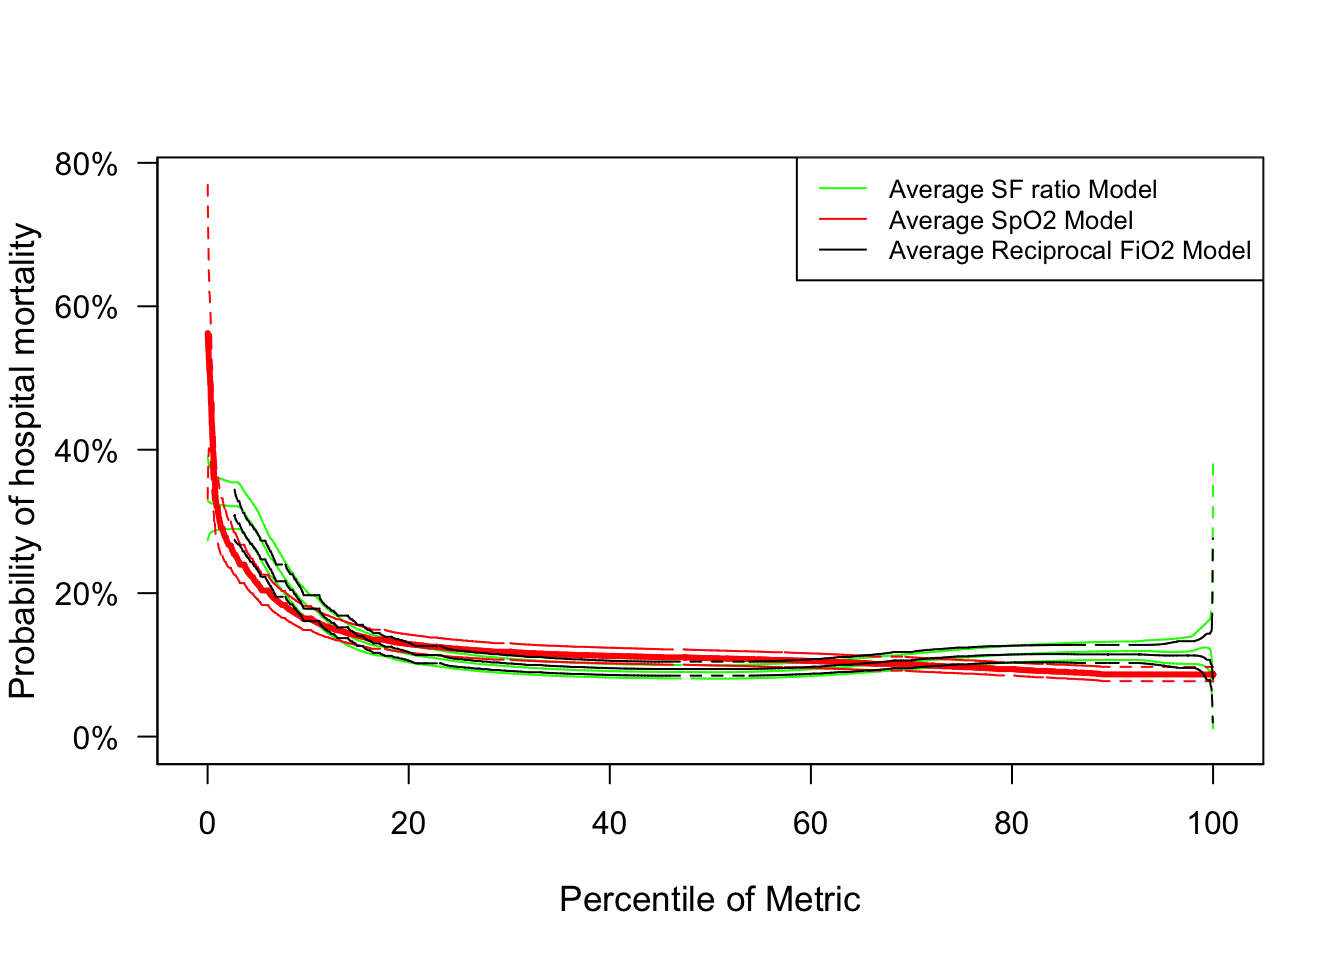
\includegraphics[width=0.9\textwidth]{figures/toratioornottoratio-4.png}
	\caption{Model Comparison: Average SF ratio vs Average \Sp vs Average \Fi}
	\label{fig:toratioornot}
\end{figure}

All three metrics are significantly correlated to patient outcome. However, as we can see from  figure \ref{fig:toratioornot} above, the SF ratio model captures both the initial down trend of the SpO2 model and some of the upward trend towards the end  FiO2 model. Therefore, we conclude that the use of the SF ratio is better as it captures part of the unique trends of both the \Sp and \Fi. 


\section{Does Transformation help?}

In using the SF ratio however, there are two concerns. First of all, the normal range of \Fi is much wider than that of \Sp. \Fi ranges from 21\% to 100\% based on the level of oxygenation provided to the patient, while \Sp only ranges from 92\% - 100\% \citep{lapum2018vital}. In taking a ratio of these two, we are concerned that the SF ratio will be more representative of \Fi than \Sp. The second concern we have is the effect that extreme values in both \Sp and \Fi might have in increasing outlier values in the SF ratio.

To check whether these concerns are indeed an issue, we consider two different transformations of the SF ratio that tackle the two concerns respectively. We test if using them shows a difference in the trend that may not have been captured by the untransformed SF ratio. The two transformations are:

\begin{enumerate}
	\item \textbf{Linear rescaling}: We rescale both the \Sp (numerator) and \Fi (denominator) to the same scale from 1 to 2 before taking the ratio and multiplying by a 100. We shall call this the Linear Rescaled SF ratio. 
	\item \textbf{Removing Extremes}: We remove the first and last percentile of 
	both the \Sp and \Fi before taking the ratio we shall call this No-Extreme SF ratio. 
\end{enumerate} 

We again plot the percentile of each metric to the probability of mortality and its 95\% confidence interval as predicted by each model. 

\begin{figure}[H]
	\centering
	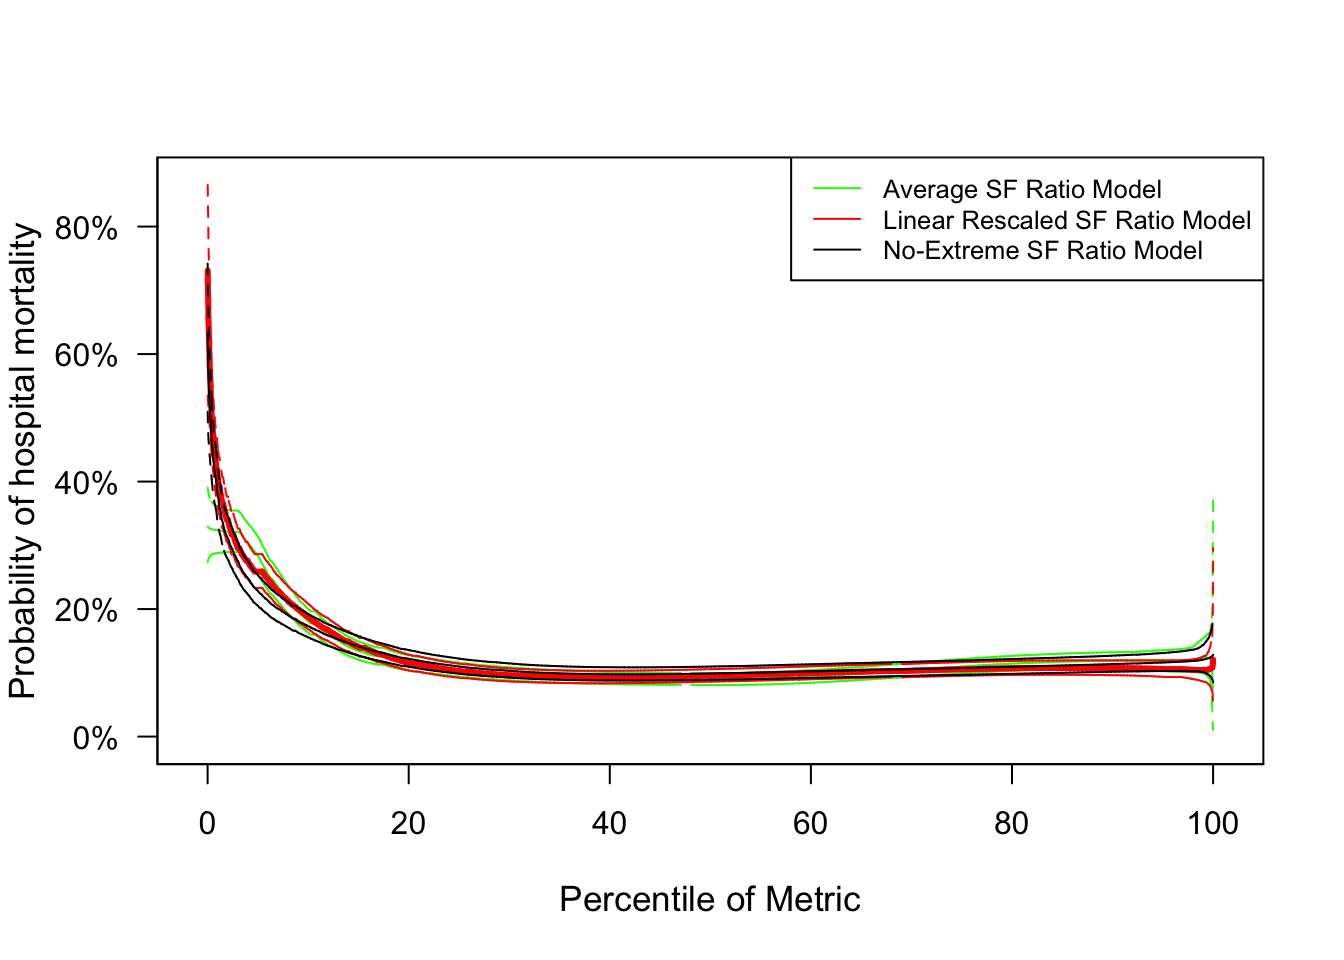
\includegraphics[width=0.9\textwidth]{figures/doestransformationhelp-4.png}
	\caption{Model Comparison: Average SF ratio vs Linear Rescaled SF ratio vs No-Extreme SF ratio}
	\label{fig:toratioornot}
\end{figure}

As the plot above suggests, all three models almost exactly coincide in predicting the confidence interval of the response variable. Therefore, it does not seem that the two suggested transformations of the SF ratio add benefit. Consequently, we will continue using the SF ratio in our models. 
\section{Timeframe of SF Ratio aggregation}


% Chapter Template

\chapter{Analysis and Findings} % Main chapter title

\label{Chapter3} % Change X to a consecutive number; for referencing this chapter elsewhere, use \ref{ChapterX}

%----------------------------------------------------------------------------------------
%	SECTION 1
%----------------------------------------------------------------------------------------




% Chapter Template

\chapter{Discussion} % Main chapter title

\label{Chapter6} % Change X to a consecutive number; for referencing this chapter elsewhere, use \ref{ChapterX}



\section{Conclusion} % Main chapter title


%----------------------------------------------------------------------------------------
%	SECTION 1
%----------------------------------------------------------------------------------------

To summarize our main results, we have found that average SF ratio over the first 24 hours of ICU stay (SF ratio) is significantly correlated with patient outcome, with the risk of  mortality significantly increasing at values of SF ratio below 180. Furthermore, the risk is exacerbated for patients on invasive mechanical ventilation than in those on non-invasive mechanical ventilation. 

We believe that this provides compelling reason to conduct further studies that examine our covariate of choice - average SF ratio over the first 24 hours of ICU stay - as a direct predictor of patient outcome. We hope that we have contributed to the field through our study. 


\section{Limitations}

%------------------------------------------------------------------------------

First of all, our study is an observational study (OS) based on retrospective data. As such, we do not control which patients get assigned what treatment methods, such as the type of mechanical ventilation. This is in contrast with a randomized controlled trial (RCT) where patients are randomly picked in order to ensure representation of the target population. In other words, in an OS, there are large observed and unobserved differences between different patient groups. This is called selection bias. Selection bias limits the generalizability of the data. 

Second, although we found significant correlation between SF ratio and mortality, we have not tested for causality. Our results, although promising, do not conclude that patient outcome is a causal effect of SF ratio. As such, the significant correlation we have established between SF ratio and mortality can only suggest for further studies that test for causality. These include the application of causal inference methods for time-varying exposure such as G-Computation to our data set \citep{snowden2011implementation} or setting up a randomized clinical trial. 
%-----------------------------------
%	SUBSECTION 2
%-----------------------------------
%
%\subsection{Subsection 2}
%Morbi rutrum odio eget arcu adipiscing sodales. Aenean et purus a est pulvinar pellentesque. Cras in elit neque, quis varius elit. Phasellus fringilla, nibh eu tempus venenatis, dolor elit posuere quam, quis adipiscing urna leo nec orci. Sed nec nulla auctor odio aliquet consequat. Ut nec nulla in ante ullamcorper aliquam at sed dolor. Phasellus fermentum magna in augue gravida cursus. Cras sed pretium lorem. Pellentesque eget ornare odio. Proin accumsan, massa viverra cursus pharetra, ipsum nisi lobortis velit, a malesuada dolor lorem eu neque.
%
%%----------------------------------------------------------------------------------------
%%	SECTION 2
%%----------------------------------------------------------------------------------------
%
%\section{Main Section 2}
%
%Sed ullamcorper quam eu nisl interdum at interdum enim egestas. Aliquam placerat justo sed lectus lobortis ut porta nisl porttitor. Vestibulum mi dolor, lacinia molestie gravida at, tempus vitae ligula. Donec eget quam sapien, in viverra eros. Donec pellentesque justo a massa fringilla non vestibulum metus vestibulum. Vestibulum in orci quis felis tempor lacinia. Vivamus ornare ultrices facilisis. Ut hendrerit volutpat vulputate. Morbi condimentum venenatis augue, id porta ipsum vulputate in. Curabitur luctus tempus justo. Vestibulum risus lectus, adipiscing nec condimentum quis, condimentum nec nisl. Aliquam dictum sagittis velit sed iaculis. Morbi tristique augue sit amet nulla pulvinar id facilisis ligula mollis. Nam elit libero, tincidunt ut aliquam at, molestie in quam. Aenean rhoncus vehicula hendrerit.


%----------------------------------------------------------------------------------------
%	BIBLIOGRAPHY
%----------------------------------------------------------------------------------------

\printbibliography[heading=bibintoc]

%----------------------------------------------------------------------------------------
%	THESIS CONTENT - APPENDICES
%----------------------------------------------------------------------------------------

\appendix % Cue to tell LaTeX that the following "chapters" are Appendices

% Include the appendices of the thesis as separate files from the Appendices folder
% Uncomment the lines as you write the Appendices

% % Appendix A

\chapter{Other Figures} % Main appendix title

\label{AppendixA} % For referencing this appendix elsewhere, use \ref{AppendixA}

\begin{figure}[H]
  \centering
    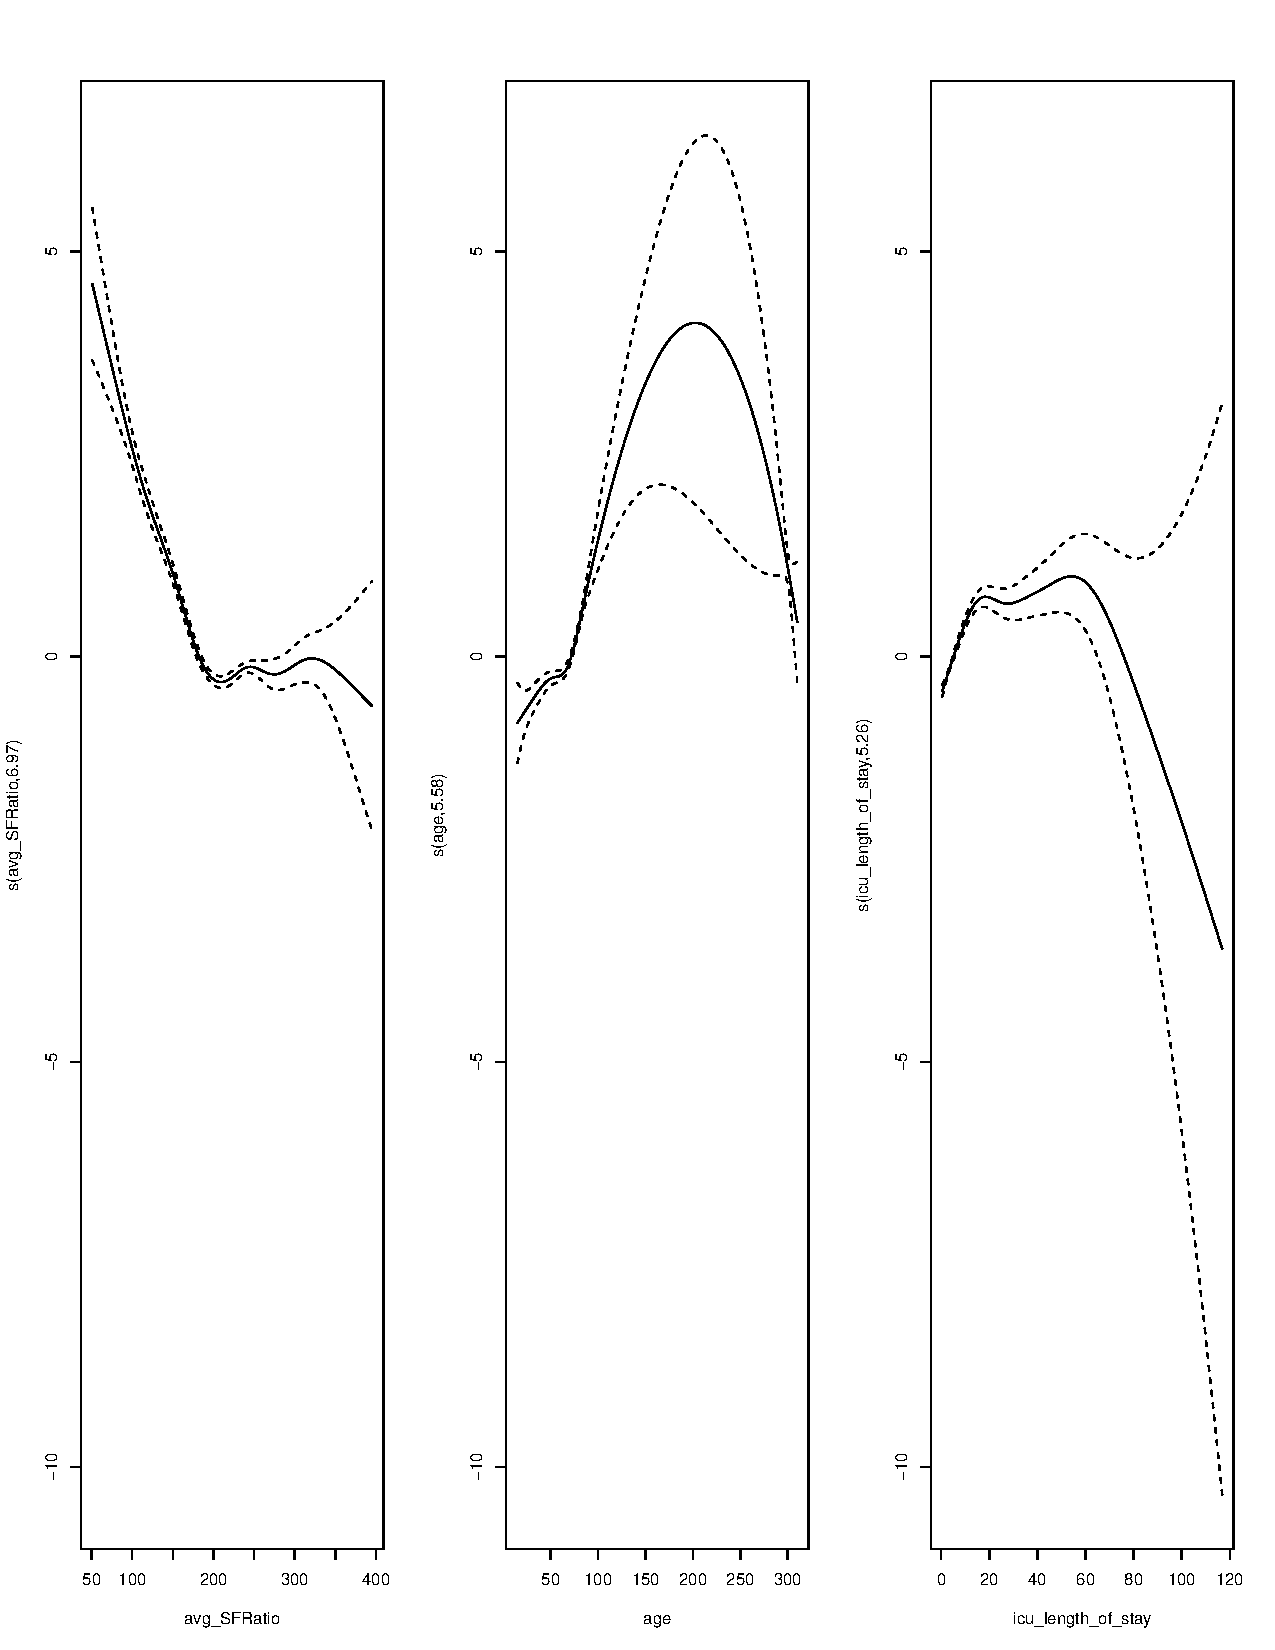
\includegraphics[width=0.9\textwidth]{figures/GAM.pdf}
  \caption{Results of GAM model}
  \label{fig:GAM_All}
\end{figure}


 % Appendix A

\chapter{Other Figures} % Main appendix title

\label{AppendixA} % For referencing this appendix elsewhere, use \ref{AppendixA}

\begin{figure}[H]
  \centering
    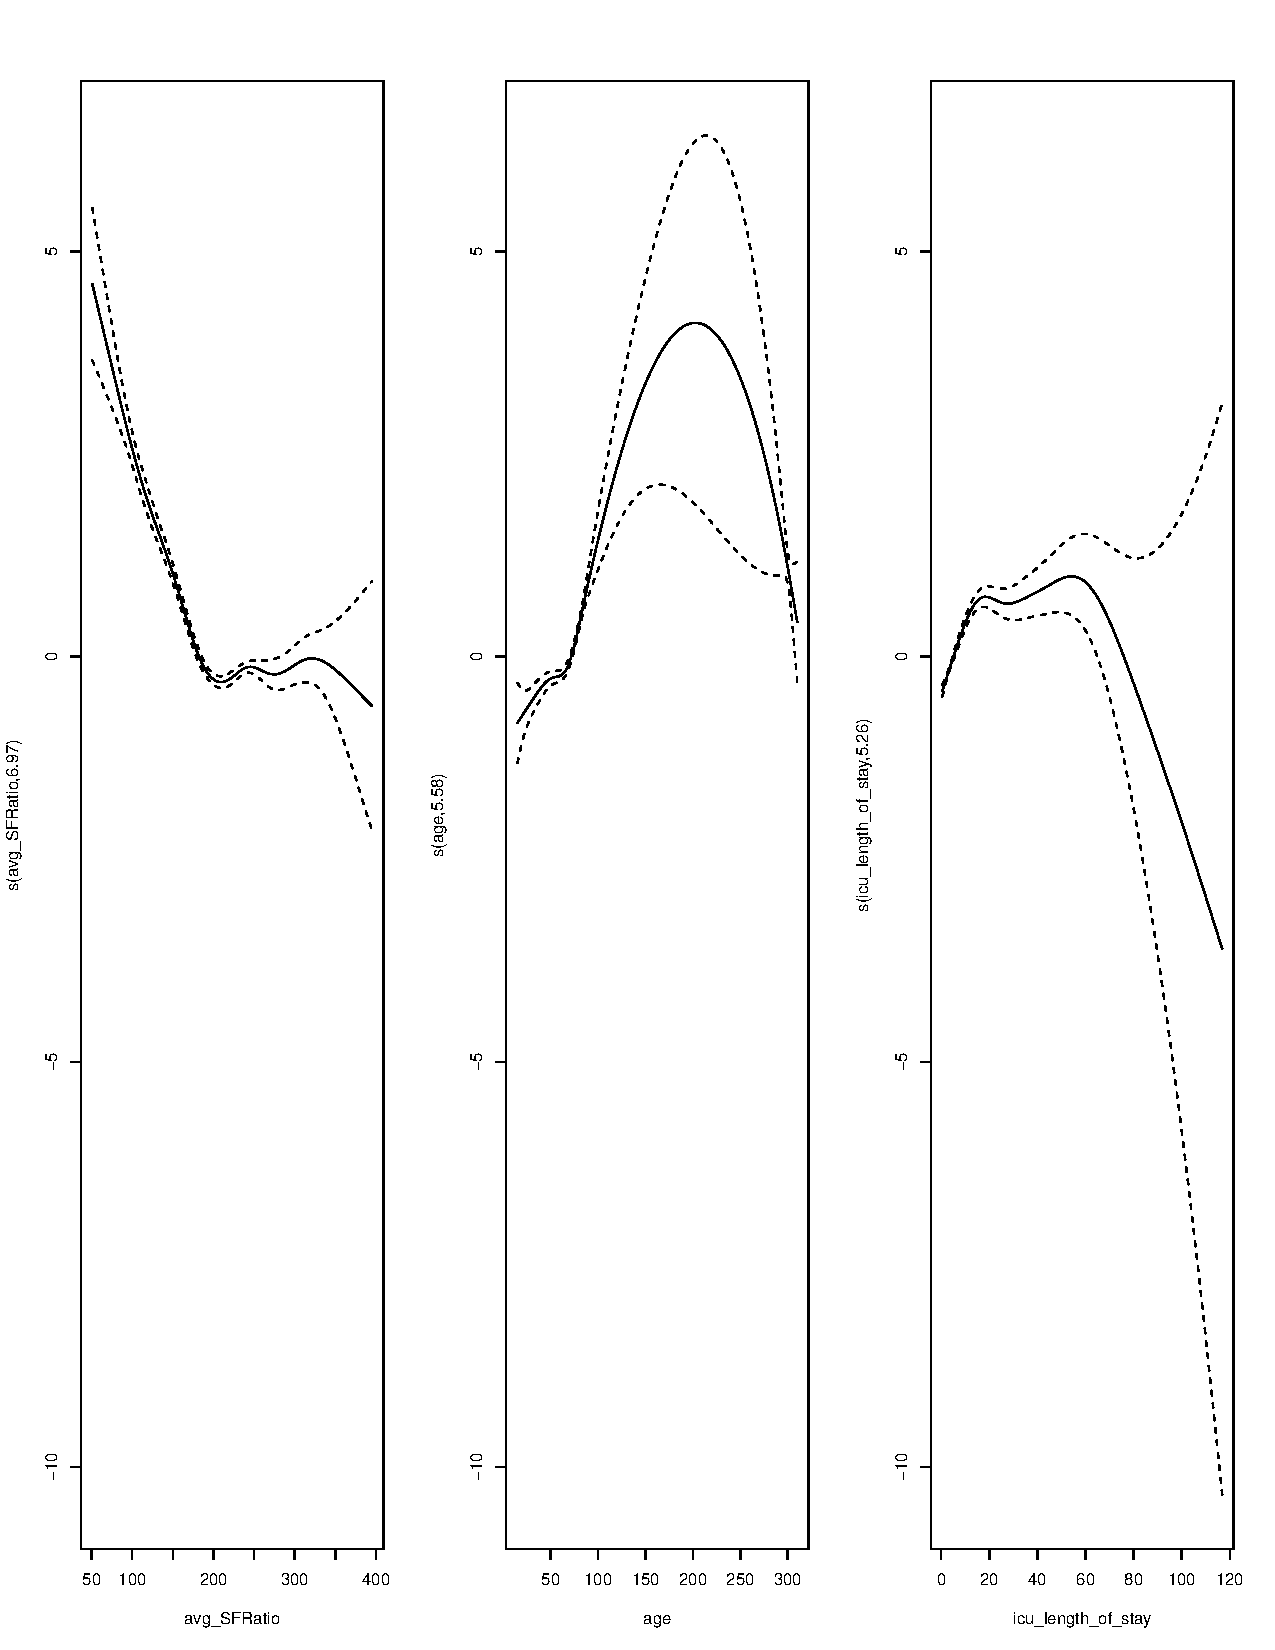
\includegraphics[width=0.9\textwidth]{figures/GAM.pdf}
  \caption{Results of GAM model}
  \label{fig:GAM_All}
\end{figure}



%----------------------------------------------------------------------------------------

\end{document}
